\lecture{26}{The Einstein and Debye Models of Solids}{Qiang Zhu}{scribe-name1,2,3}

\section{Einstein Model}
The Einstein Model of a solid crystal is expressed as an independent three dimensional harmonic oscillator.
The multiplicity of an Einstein solid containing $N$ oscillators and $q$ energy units is approximately
\begin{equation} 
\Omega(N, q) \approx (\frac{q+N}{q})^q (\frac{q+N}{N})^N
\end{equation}
Starting with this formula, the entropy could be expressed as 
\begin{equation} 
\begin{split}
S = k\textrm{ln}\Omega &= k\textrm{ln}(\frac{q+N}{q})^q + k\textrm{ln}(\frac{q+N}{N})^N\\
                       &= kq\textrm{ln}(\frac{q+N}{q}) + kN\textrm{ln}(\frac{q+N}{N})
\end{split}
\end{equation}

Let us express the energy as $U = q\epsilon$ 
\begin{equation}
\begin{split}
\frac{1}{T} &= \frac{\partial S}{\partial U} = \frac{1}{\epsilon}\frac{\partial S}{\partial q} \\
            &= \frac{k}{\epsilon} \frac{\partial}{\partial q}[q\textrm{ln}(q+N) - q\textrm{ln}q + N\textrm{ln}(q+N) - N\textrm{ln}N] \\
            &= \frac{k}{\epsilon} [\textrm{ln}(q+N) + \frac{q}{q+N} - \textrm{ln}q  - \frac{q}{q} +  \frac{N}{q+N} + 0] \\
            &= \frac{k}{\epsilon} [\textrm{ln}\frac{q+N}{q} + \frac{q+N}{q+N} - \frac{q}{q}] \\
            &= \frac{k}{\epsilon} \textrm{ln}\frac{q+N}{q} 
\end{split}
\end{equation}
So the $U$ can be expressed as follows
\begin{equation}
U = \frac{N\epsilon}{e^{\epsilon/kT}-1}
\end{equation}

The heat capacity is therefore
\begin{equation}
C_V =  \frac{\partial U}{\partial T} 
    = -\frac{N\epsilon}{(e^{\epsilon/kT}-1)^2} \frac{\partial e^{\epsilon/kT}}{\partial T} 
    =  \frac{N\epsilon^2}{kT^2} \frac{e^{\epsilon/kT}}{(e^{\epsilon/kT}-1)^2}
    =  Nk \frac{ (\epsilon/kT)^2  e^{\epsilon/kT}}{(e^{\epsilon/kT}-1)^2}
\end{equation}

When $kT \gg \epsilon$,
\begin{equation}
C_V = \frac{N\epsilon^2}{kT^2} \frac{1+ \epsilon/kT} {(\epsilon/kT)^2} = Nk
\end{equation}
Remember we would have 3$N$ oscillators for $N$ atoms, therefore $C_V = 3Nk$.
This exactly follows the equipartition theorem. 

Below $kT \approx \epsilon$, the heat capacity falls off, approaching zero as the temperature goes to zero. This prediction generally agrees with experiment but not in detail. The equation predicts $C_V$ exponentially goes to 0, when T $\rightarrow$ 0. But experiments show that the true low-temperature behavior is cubic: $C_V \propto T^3$. The problem with the Einstein model is that the atoms in a crystal do not vibrate independently of each other. Therefore a better assumption is needed.

\section{Debye Model}
In reality, there should be low-frequency modes of oscillation in which large groups of atoms are moving together, and also high-frequency modes in which atoms are moving opposite to their neighbors.
The units of energy come in different sizes, proportional to the frequency of the modes of the vibration. Even at very low temperatures, a few low-frequency modes are still active. 
This is the reason why the heat capacity goes to 0 less dramatically than the prediction by the Einstein model.

Based on this reasoning, Debye proposed that each mode of oscillation has a set of equally spaced energy levels with the unit of energy equal to
\begin{equation}
\epsilon = hf = \frac{hc_s}{\lambda}=\frac{hc_sn}{2L}
\end{equation}
Where $L$ is the length of crystal, $n$ is the magnitude of the vector in $n$-space specifying the shape of the wave, and $c_s$ is the speed of the wave.

When the mode is in equilibrium at temperature $T$, the number of units of energy is given by the Plank distribution:
\begin{equation} 
\bar{n} = \frac{1}{e^{\epsilon/kT}-1}
\end{equation} 
We can think of these units of energy as particles obeying the Bose-Einstein statistics with $\mu$=0. These particles are called {\emph phonons}.

To calculate the total thermal energy, we add up the energies of all allowed modes:
\begin{equation}
U = 3\sum_{n_x}\sum_{n_y}\sum_{n_z} \epsilon \bar{n}(\epsilon)
\end{equation}
The factor of 3 counts the three polarization states for each polarization states for each $\bar{n}$.

In a crystal, the atomic spacing puts a strict lower limit on the wavelength. $n$ cannot exceed the number of atoms in a row. If the 3D crystal 
is a cube, the $n$ along any direction is $N^{\frac{1}{3}}$, where $N$ is the total volume.

Summing over a cube depends on $n_x$, $n_y$ and $n_z$ in a very complicated way. Debye got the idea to pretend that the relevant region of $n$-space is 
a sphere. He chose a sphere whose total volume is $N$. You can easily show that the radius of the sphere has to be
\begin{equation}
n_\textrm{max} = (\frac{6N}{\pi})^{1/3}
\end{equation}

Physical explanations:
\begin{enumerate}
\item At high $T$, only the total number of modes matters.
\item At low $T$, modes with large $\bar{n}$ are frozen out anyway.
\item In the intermediate region, not exact, but a continuous function.
\end{enumerate}

Therefore, we apply the Debye's approximation and convert the sums to integrals in spherical coordinates,
\begin{equation}
U = 3 \int_0^{n_\textrm{max}} dn \int_0^{\pi/2} d\theta \int_0^{\pi/2} d\phi n^2\textrm{sin}\theta \frac{\epsilon}{e^{\epsilon/kT}-1}
\end{equation}
Since the angular integrals gives $\pi/2$, leaving us with
\begin{equation}
U = \frac{3\pi}{2} \int_0 ^{n_\textrm{max}} \frac{hc_s}{2L} \frac{n^3}{e^{hc_sn/2LkT}-1} dn
\end{equation}

Let's make a substitution,
\begin{equation}
x = \frac{hc_sn}{2LkT}
\end{equation}

Then 
\begin{equation}
x_\textrm{max} = \frac{hc_s n_{\textrm{max}}}{2LkT} = \frac{hc_s}{2kT} (\frac{6N}{\pi V})^{1/3} = \frac{T_D}{T}
\end{equation}
$T_D$ is the Debye Temperature, a characteristic temperature. 

After substitution, we get
\begin{equation}
U = \frac{9NkT^4}{T_D^3} \int _0 ^{T_D/T} \frac{x^3}{e^x -1} dx
\end{equation}

When $T \gg T_D$, the upper limit of the integral is much less than 1, so $x$ is always very small, and we 
can approximate $e^x \approx 1+x$. Then 1 cancels, and the integral is simply $x^2dx$, leading to the final result
\begin{equation}
 U = \frac{9NkT^4}{T_D^3} \frac{1}{3} (\frac{T_D}{T})^3 = 3NkT
\end{equation}

When $T \ll T_D$, the upper limit goes to infinity, and the integral gives a constant of $\pi^4/15$, so the total energy is
\begin{equation}
U = \frac{3\pi^4}{5} \frac{NkT^4}{T_D^3}
\end{equation}
And the heat capacity becomes proportional to $T^3$.

The prediction agrees very well with low-temperature observations. However, for metal there is linear contribution from the conduction electrons.
\begin{equation}
C = \gamma T + \frac{12\pi^4Nk}{5T_D^3} T^3,
\end{equation}

where $\gamma$ is a dimensionless coefficient. The Debye temperature ranges from 88 K for lead to 1860 K for diamond. Since the heat capacity reaches 95 of its maximum value at $T=T_D$, the Debye
temperature gives you a rough idea of when you can get away with just using the equipartition theorem. 

The Debye model gives you a rough idea still. For a more rigorous analysis, one needs to know exactly the distribution of phonons, which belongs
to a book in solid state physics.

\section{Further Discussions}
\begin{enumerate}
\item{Both Einstein and Debye models give the correct high temperature limit. It indicates that all oscillators under high $T$ essentially have the same energy, even though the oscillators follow that Bose-Einstein distribution in the Debye model. Try to apply the distribution model to prove it.}
\item{In low temperature limit, the Debye model captures the right physics, but why does it fail in the intermediate temperature? In the Debye model, it assumes that the
oscillators with lower frequencies have more populations, and the phonon numbers monotonically decrease with the increase of frequency. Not true in reality!}


\begin{figure}[h]
\centering
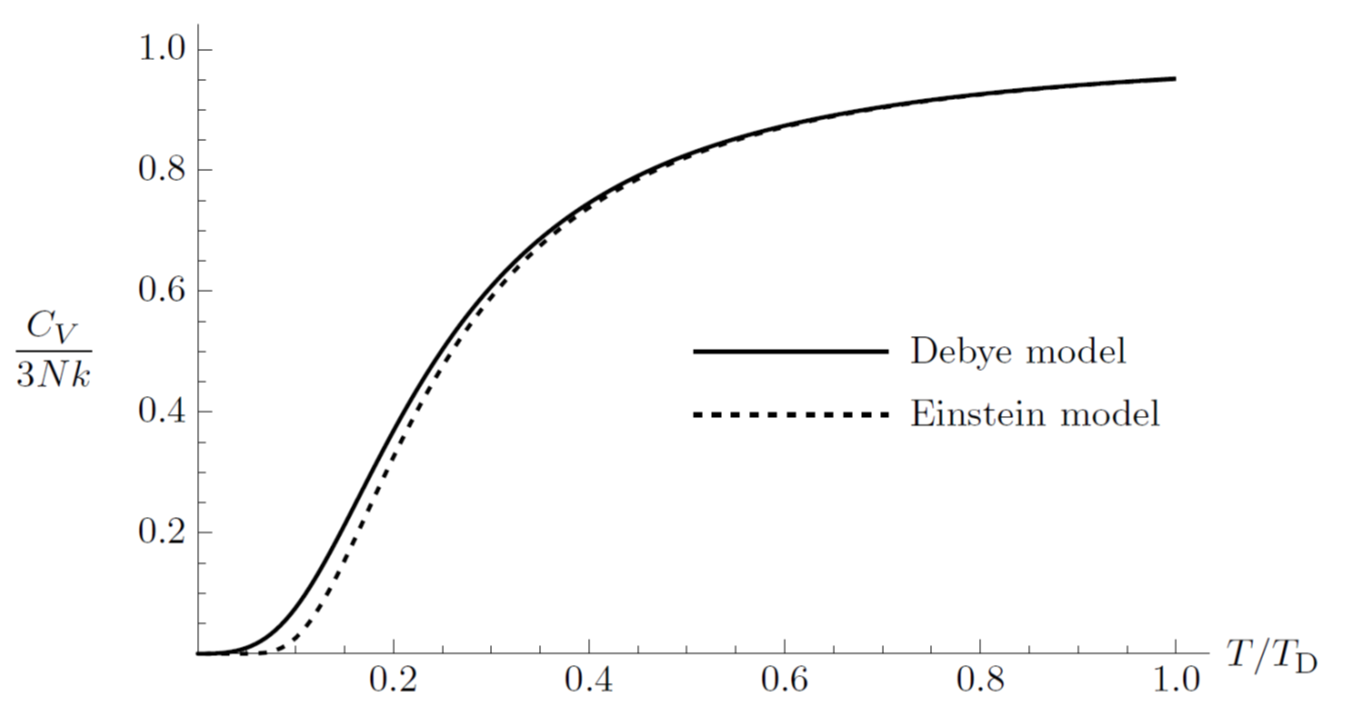
\includegraphics[width=0.9\linewidth]{imgs/Debye.png}
\caption{The Debye prediction for the heat capacity of a solid, with the
prediction of the Einstein model plotted for comparison. The constant ⇤ in the
Einstein model has been chosen to obtain the best agreement with the Debye
model at high temperatures. Note that the Einstein curve is much flatter than the Debye curve at low temperatures. Copyright 2000, Addison-Wesley. }
\end{figure}

\end{enumerate}



